\documentclass[11pt]{article}

\usepackage[margin=1in]{geometry}
\usepackage{amsmath}
\usepackage{graphicx}
\usepackage{subcaption}
\usepackage{float}

\title{CSE 242 Assignment 3}
\author{Nicholas Mo (1997187)}
\date{}

\begin{document}

\maketitle

\section*{Question 1: Hard-margin SVM}

\begin{figure}[H]
  \centering
  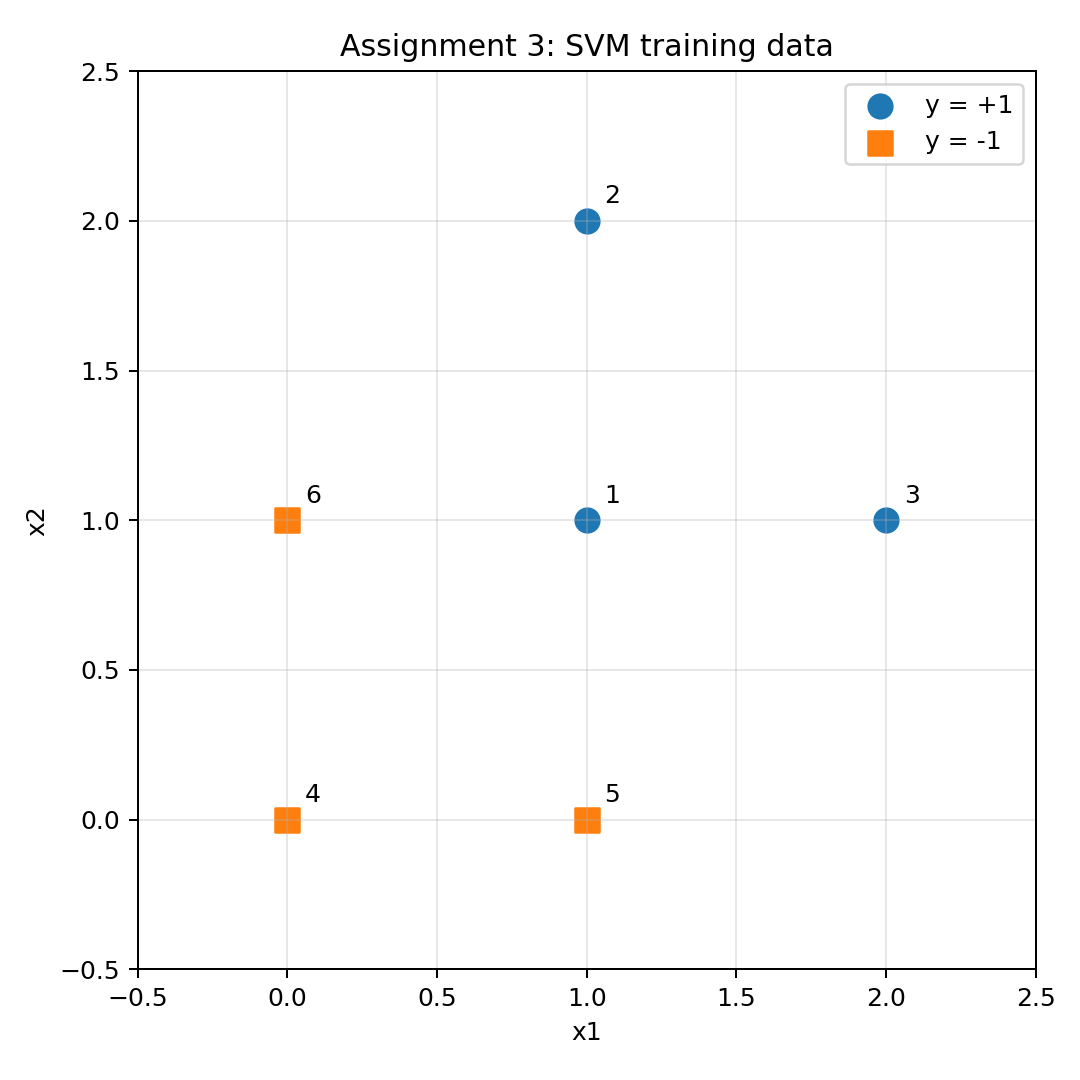
\includegraphics[width=0.45\textwidth]{figures/svm_data.png}
\end{figure}

\textbf{(a)} The support vectors are \textbf{points 1, 5, and 6}. Point 1 $(1,1)$ is the positive point closest to the negatives, and points 5 $(1,0)$ and 6 $(0,1)$ are the negatives closest to it. Points 2, 3, and 4 are farther from the gap, so they don't affect the boundary.

\textbf{(b)} Support vectors satisfy $\mathbf{w} \cdot \mathbf{x}_i + b = y_i$:
\begin{align*}
  \text{Point 1:} &\quad w_1 + w_2 + b = 1 \\
  \text{Point 5:} &\quad w_1 + b = -1 \\
  \text{Point 6:} &\quad w_2 + b = -1
\end{align*}
Subtracting the second and third equations from the first gives $w_2 = 2$ and $w_1 = 2$, so $b = -3$. The boundary is
\[
  2x_1 + 2x_2 - 3 = 0.
\]
All other points satisfy $y_i(\mathbf{w} \cdot \mathbf{x}_i + b) = 3 \geq 1$, so the constraints hold.

The geometric margin (distance from the boundary to the closest points) is
\[
  \frac{1}{\lVert \mathbf{w} \rVert} = \frac{1}{2\sqrt{2}} \approx 0.354.
\]
The full width between the supporting lines is $2/\lVert \mathbf{w} \rVert \approx 0.707$.

\section*{Question 2: K-means}

\textbf{(a)} Each point is assigned to the nearest centroid by squared Euclidean distance; ties go to the lowest centroid index. Each centroid is then updated to the mean of its points. An empty cluster keeps its previous centroid.

\textbf{(b)}

\begin{figure}[H]
  \centering
  \begin{subfigure}{0.32\textwidth}
    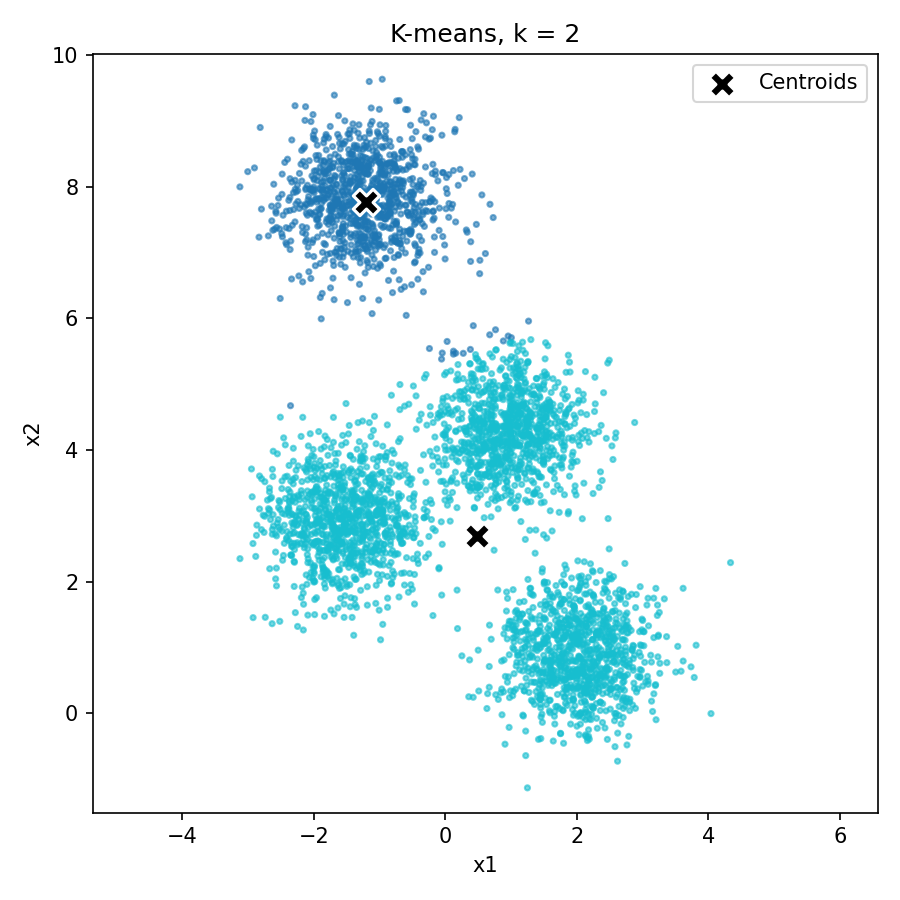
\includegraphics[width=\linewidth]{figures/kmeans_k2.png}
  \end{subfigure}
  \begin{subfigure}{0.32\textwidth}
    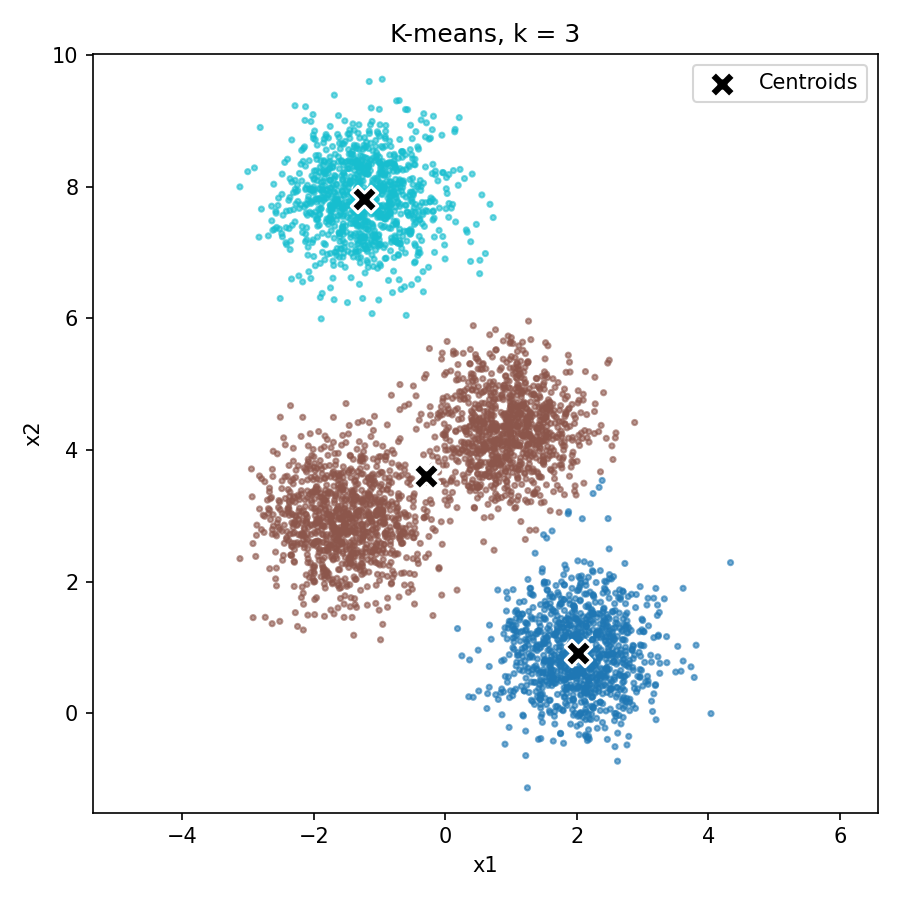
\includegraphics[width=\linewidth]{figures/kmeans_k3.png}
  \end{subfigure}
  \begin{subfigure}{0.32\textwidth}
    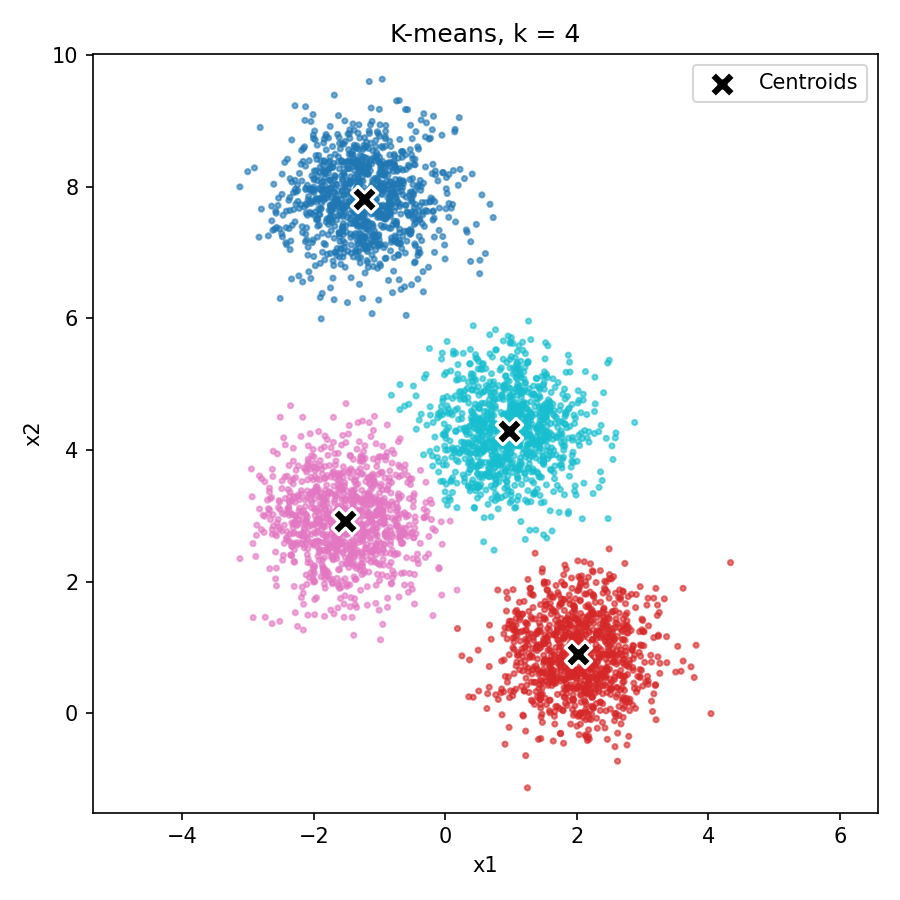
\includegraphics[width=\linewidth]{figures/kmeans_k4.png}
  \end{subfigure}

  \begin{subfigure}{0.32\textwidth}
    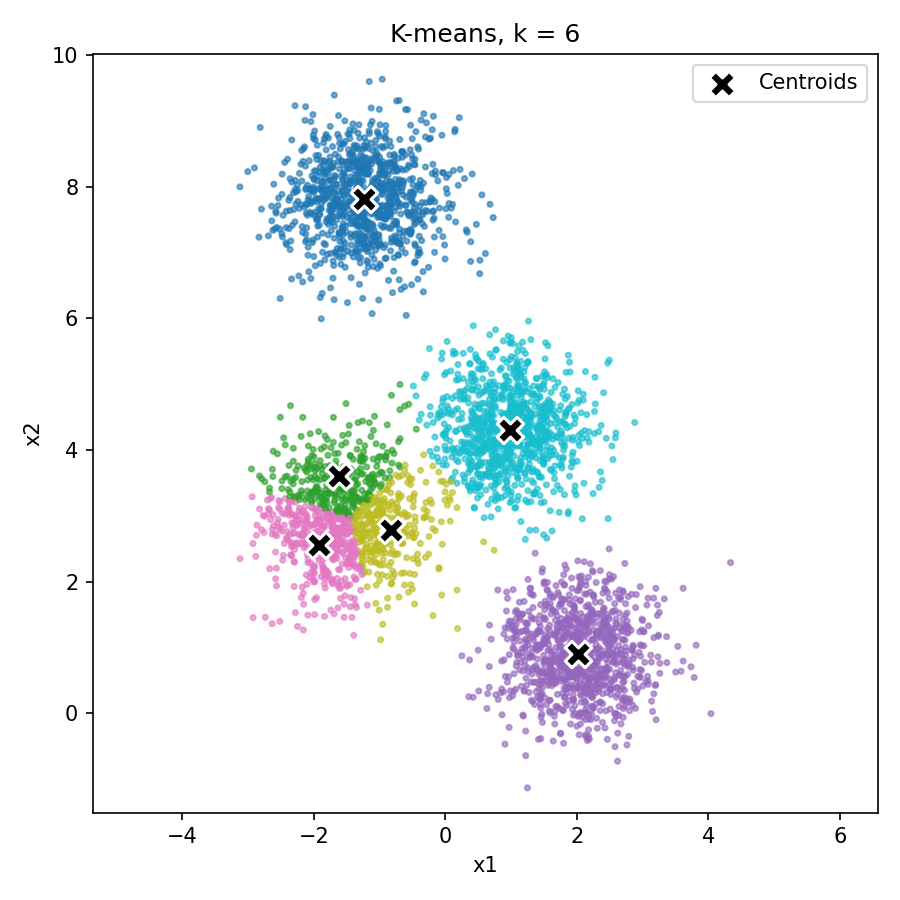
\includegraphics[width=\linewidth]{figures/kmeans_k6.png}
  \end{subfigure}
  \begin{subfigure}{0.32\textwidth}
    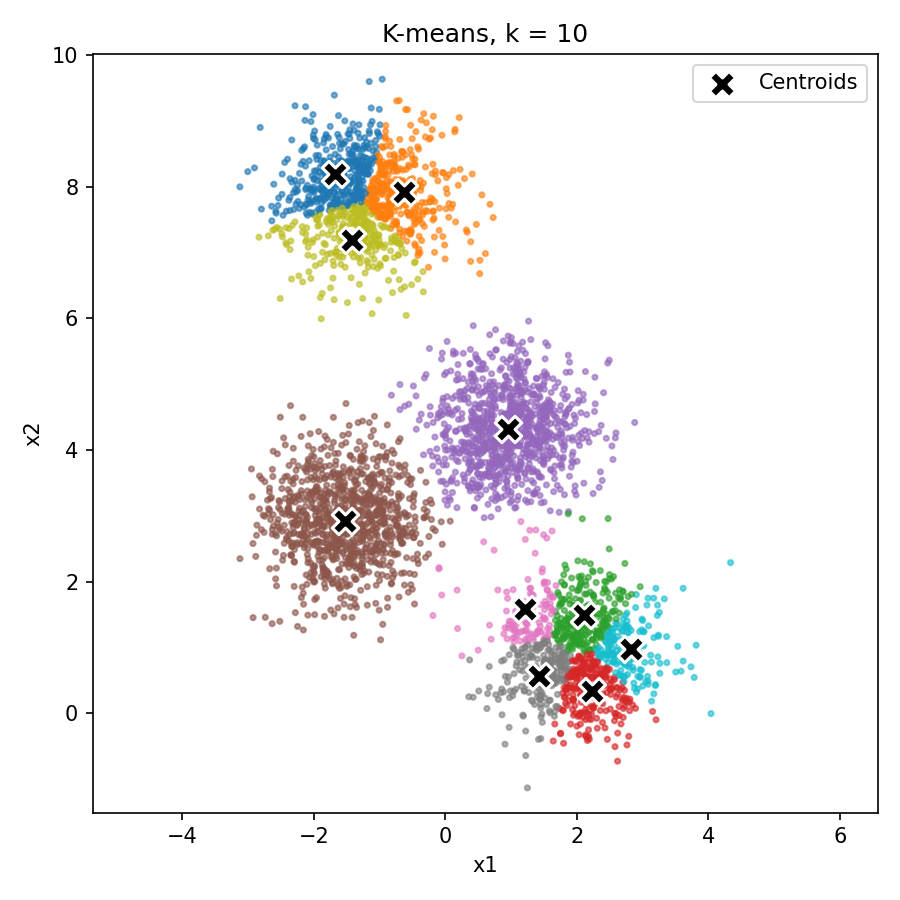
\includegraphics[width=\linewidth]{figures/kmeans_k10.png}
  \end{subfigure}
\end{figure}

With $k = 2$ and $k = 3$, there are fewer clusters than blobs, so nearby blobs get merged. At $k = 4$, the clusters match the four generating blobs almost exactly. With $k = 6$ and $k = 10$, K-means starts splitting real blobs into pieces, and where those splits happen depends on the initial centroids rather than any real structure in the data.

\section*{Question 3: Noisy labels and K-NN repair}

Over 20 trials (seed 0):

\begin{center}
  \begin{tabular}{lc}
    \hline
    Method & Mean test accuracy \\
    \hline
    Baseline (noisy labels) & 0.8280 \\
    K-NN repair & 0.8644 \\
    \hline
    Difference & +0.0364 \\
    \hline
  \end{tabular}
\end{center}

K-NN repair helped, improving accuracy in all 20 trials. Because positive labels are flipped more often than negative ones, the baseline SVM is biased toward predicting negative. Majority voting among neighbors fixes many of the scattered wrong labels, which removes most of that bias. It could hurt near the class boundary, where neighbors are mixed and correct labels can get overwritten, or if the noise were clustered so a whole neighborhood shared the wrong label. Per-trial results are in \texttt{noise\_comparison.csv}.

\section*{Acknowledgment}

I used Claude (Anthropic) to write the code, derive the SVM solution, and draft this write-up. I reviewed and ran the code and checked the results. The session transcript is attached.

\end{document}
